\section{Introduction}
Deep convolutional neural networks are currently the leading technique for image classification.
Convolutional layers capture patterns with spatial locality, while deep topologies capture the compositional nature of images.
The problem of \emph{video} classification introduces a new, temporal dimension not leveraged by typical 2D CNNs. For instance, a video of a human subject may contain temporal concepts such as gestures or gait that cannot be extracted from a single frame. This prompts the question:
 how can we best capture the additional information contained within this temporal dimension?   

There are indeed methods of preprocessing temporal information into a single 2-dimensional input~\cite{brox}, but a more attractive research goal is to develop a neural network that can discover temporal relationships on its own.
There are multiple recent approaches towards this goal, but as of yet no consensus on which is superior.

The difficulties in training neural networks on video input include the following: memory requirements (particularly if 3D convolutions are used), fewer public data sets, size of the data sets (for instance, the Sports-1M data set is $\approx 4TB$ large), and a lack of consensus on which structural approaches are most effective.

In just the last two years, a variety of techniques have been investigated, including 3-dimensional convolutional neural networks (3D-CNN) and Long Short-Term Memory (LSTM). Additional techniques have been incorporated within these strategies, such as slow-fusion, optical-flow, and retraining of pre-trained ImageNet networks.

The purpose of this project is to examine and compare these approaches, while comparing to an additional, novel technique that we introduce that uses a second CNN layer to extract temporal information from sequentially-generated ImageNet vectors. 

We make the following contributions:
\begin{enumerate}
\item Implement and analyze a 2D-CNN $\to$ LSTM architecture for video classification.
\item Introduce and analyze a novel 2D-CNN $\to$ 2D-CNN architecture for video classification. 
\item Investigate the effect of replacing the first CNN with novel ImageNet architectures.
\end{enumerate}

\section{Background}
Insert background here.
%Summarize and cite

Describe LSTM~\cite{lstm}.

Describe ImageNet (Citation for VGG-net~\cite{vggnet} and ResNet~\cite{resnet})

Describe Slow Fusion~\cite{cnnvid}

Describe Optical Flow~\cite{brox}

Describe LSTM applied to feature vectors~\cite{}

\subsection{Related Work}
%What has been done in similar fields/problems? What are the limitations of current approaches?
%Recurrent long-term convolutional models are most frequently used in speech and language applications, but it is possible to apply them to visual time-series data. 
One popular approach is to apply a 2D-CNN to each frame of the video, followed by an RNN with LSTM~\cite{ltrcn}. 
Another approach is slow-fusion, which applies multiple frames to the input at the same time~\cite{cnnvid}. This approach, applied to a simply CNN, shows only a modest improvement over CNN single-frame learning.
Tran, et al. demonstrated that using 3D-CNNs instead of 2D can achieve state-of-the-art results on several data sets~\cite{stf}.
Ng, et al. demonstrate that instead of training on `short snippets' (such as in~\cite{cnnvid,stf}), an LSTM approach allows us to train on entire videos efficiently~\cite{snip}, and achieves state-of-the-art performance on several data sets. Furthermore, Hu, et al \cite{cnnMNLS} demonstrate in natural language processing that instead of using another RNN (or LSTM), CNN can also be used as temporal encoder to extract sequence of information from sentenses. 

Many of these papers incorporate additional features such as optical flow~\cite{brox} and improved dense trajectory, both of which involve optimization techniques applied to subsets of frames. 
\section{Approach and Techniques}
%What is your proposed approach to solving the problem? How does it compare to existing approaches?
%Note: It's OK for these projects to be similar to existing approaches, although if you want to publish the results they will have to have some novelty.
We have decided on combining two possible approaches, which address
the third, temporal dimension in different ways: Convolutional Neural
Networks (3D-CNNs or CNN as temporal encoder)~\cite{stf,cnnvid,cnnMNLS} and Long
Short-Term Memory /Recurrent Neural Networks (Regular or Multi-dimensional LSTM)~\cite{ltrcn}. 

\subsection{Baseline}
Our baseline model applies a standard pretrained ImageNet CNN to each of the input frames. A simple averaging process is used on the set of output vectors to produce a predicted class-- essentially implementing a vote. This is shown in~\reffig{fig:cnn}. 
\begin{figure}
  \centering
  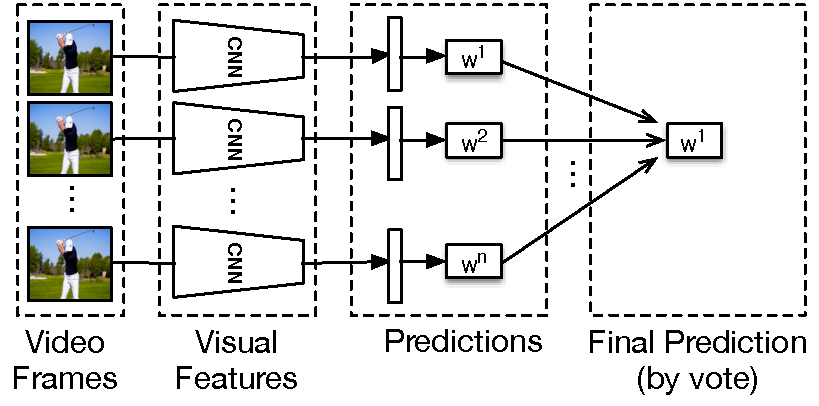
\includegraphics[width=1.0\linewidth]{figs/cnn}
  \caption{Static CNN Network}
  \label{fig:cnn}
\end{figure}

\subsection{3D CNN}
% 3D-CNNs
Using a 3D Convolutional Neural Network, it is possible to build a classifier on a moving window
of frames using 3D convolutions to extract useful local movement information. However, 3D-CNNs introduce a massive memory blowup that may make training infeasible on GPUs.
To address this, we would like to use the slow-fusion model~\cite{cnnvid} instead of 3D kernels. In addition, we also plan to apply 3D kernels to one or two layers to check the improvement if we don't meet the memory problem.


% LSTM
\subsection{RNN-LSTM}
An LSTM/RNN approach is able to build the classifier with long term memory using a much larger number of frames at once. Combining a slow-fusion CNN with LSTM would combine the local movement information with long-term memory, with possible gains in learning. This approach is illustrated in~\reffig{fig:lcrn}.
\begin{figure}
  \centering
  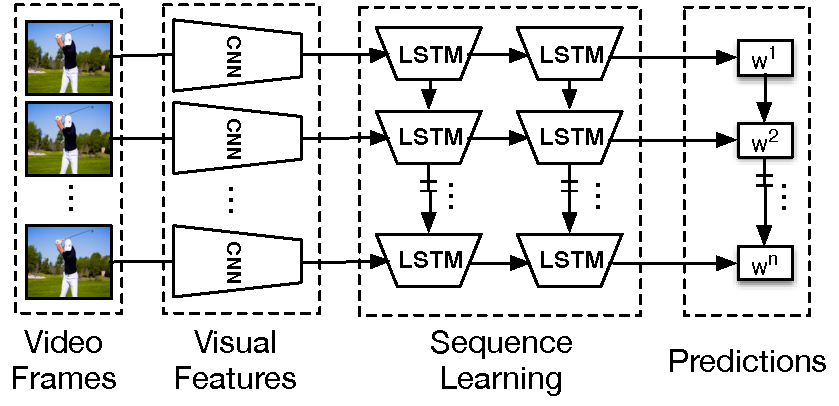
\includegraphics[width=1.0\linewidth]{figs/lcrn}
  \caption{LRCN Network}
  \label{fig:lcrn}
\end{figure}
Furthermore, the current LSTM model is built on the fully-connected
layer, which does not conserve spatial information. We would like to examine the 
effectiveness of adding the LSTM network at earlier layers.
If we apply LSTM directly after the convolution layer,
the input to LSTM model is actually multi-dimensional tensor. To address
this challenge, we would like to apply the multi-dimensional LSTM
\cite{byeon2015scene} to efficiently take advantage of the spatial
information following an early convolution layer. 

\subsection{Temporal CNN}
% CNN + CNN (1D convolution) ==> Yan
Other than the LSTM model for the temporal encoder, convolutional architecture(CNN) has also been applied to model sentences using a pre-trained embedding of words ~\cite{cnnSC,cnnMNLS}. We would like to implement this idea into the video classification. First, a pre-trained CNN architecture can be applied as spatial encoder to each frame to extract features. Furthermore, 1D or 2D CNN can be applied as the temporal encoder. For 1D CNN, we take 1D convolution on a sliding window of the concatenated feature vectors from the spatial decoder. For 2D CNN, we apply 2D convolution and 2D max-pooling directly on the a sliding window of the feature matrix from the spatial encoder. This approach is illustrated in~\reffig{fig:tnn}.
\begin{figure}
  \centering
  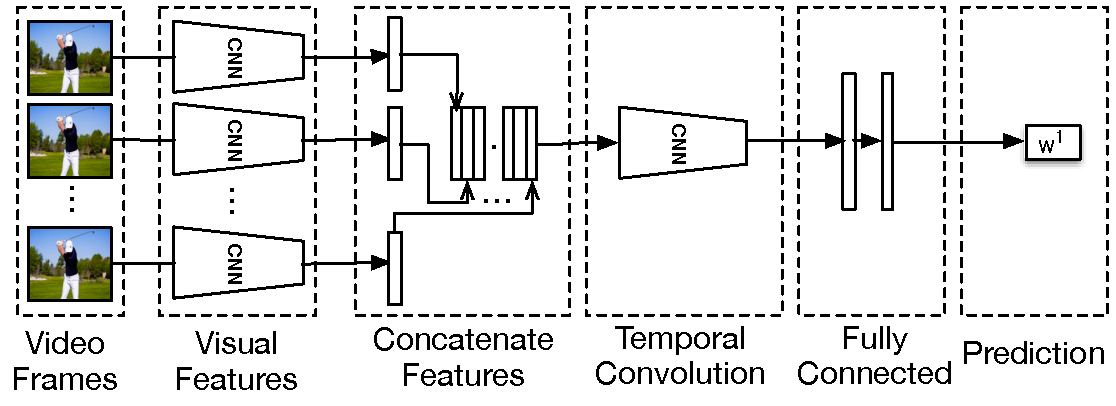
\includegraphics[width=1.0\linewidth]{figs/tnn}
  \caption{Temporal CNN Network}
  \label{fig:tnn}
\end{figure}

\section{Experiments}
\subsection{Data Set}
We propose to begin with a well-established data set such as UCF-101~\cite{ucf101}, which contains 13320 videos from 101 action categories. For early training purposes we may use only a small subset of these actions, such as a subset of 10 sports. The ultimate goal is applying our framework to Sports-1M~\cite{cnnvid}, which contains around 1 million Youtube videos belonging to 487 categories. In this way, we can compare our methods with the current state-of-the-art methods.

\subsection{Experimental Methodology}
%What specific experiments are you planning on conducting? How are they testing the specific problem you want to solve?
For training we plan to use the Jinx cluster at Georgia Tech. Each node is equipped with 2 nVidia Tesla M2090 ``Fermi'' GPU cards, and CPU nodes with large memory are available.

The following is a set of proposed experiments, some of which we have started:
\begin{itemize}
\item Move 2D-LSTM within convolution layers to see if this better incorporates spatial information.
\item Incorporate slow fusion within a 2D-CNN to see if this input approach yields higher accuracy.
\item Replace a 2D-CNN-LSTM network with a Shallow ResNet-LSTM network (with or without slow fusion)-- to see if ResNet provides significant gains over the AlexNet used by existing studies.
\item Study if slow-fusion \emph{combined} with optical-flow input provides significantly better results than either approach on its own.
\item Using CNN + LSTM as base line compare with the performance from CNN + 1D-CNN/2D-CNN.

\end{itemize}

\subsection{Results}
In~\RefFigure{fig:demo} we show an example of the video output that our model produces. The first label is the result from the TCNN model, and the second label from the LSTM model. In this case, the TCNN model made a misprediction. 
\begin{figure}
  \centering
  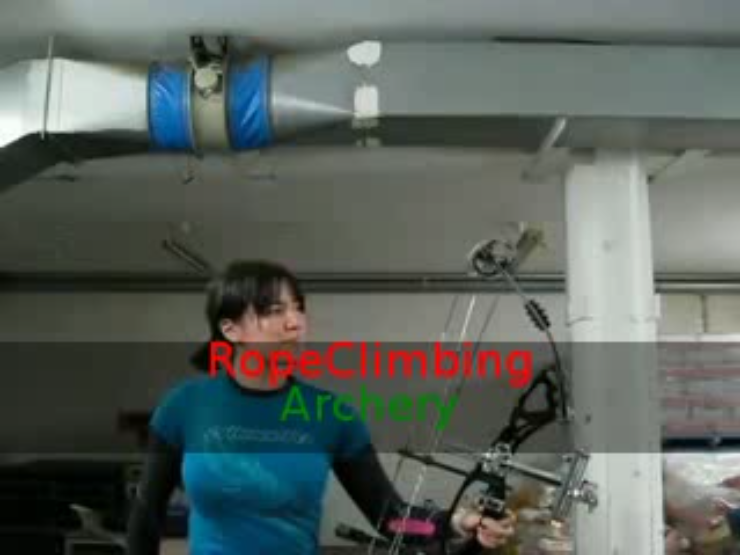
\includegraphics[width=0.8\linewidth]{figs/demo}
  \caption{Example of video output.}
  \label{fig:demo}
\end{figure}

In~\RefFigure{fig:cnntest} we see the training and testing error for the baseline model. The ResNet model performs over 10\% better than the NIN model, which is about the difference we'd expect for static image classification. 
\begin{figure}
  \centering
  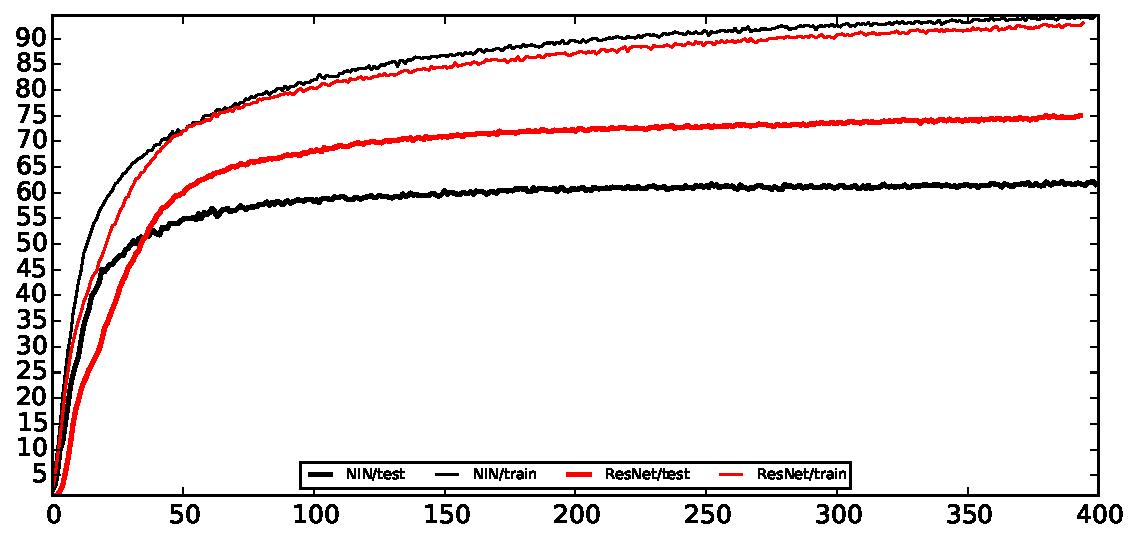
\includegraphics[width=1.0\linewidth]{figs/CNNout}
  \caption{CNN Training and Test Error}
  \label{fig:cnntest}
\end{figure}

We present the training results for the LSTM model in~\RefFigure{fig:lstmtest}. The models vary in which ImageNet model is used for the first layet. Again, we see that ResNet performs the strongest, and that the deeper ResNet networks perform incrementally better than shallower ones. 
\begin{figure}
  \centering
  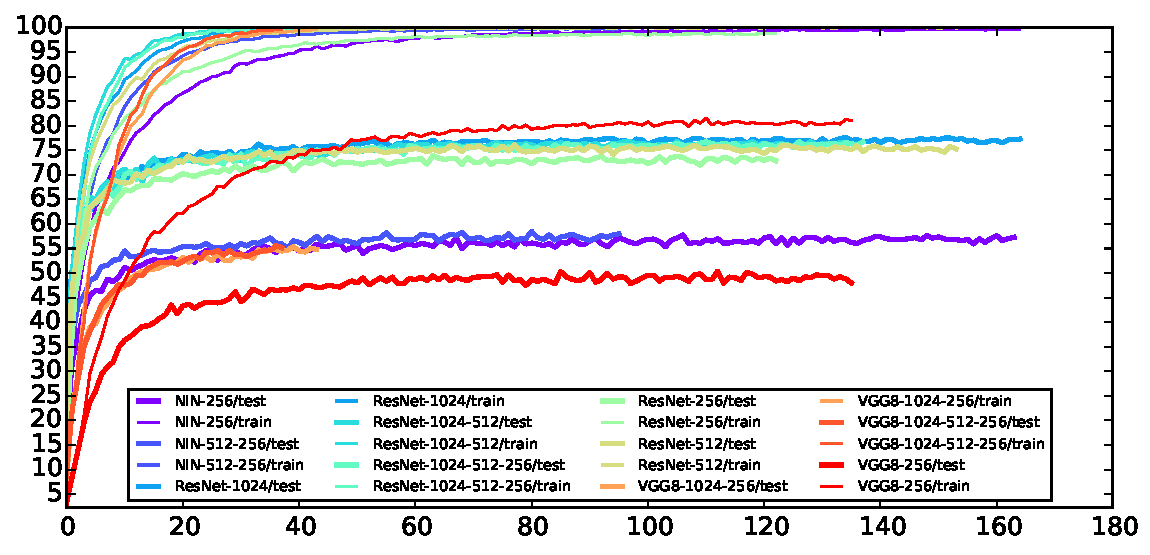
\includegraphics[width=1.0\linewidth]{figs/RNNout}
  \caption{LSTM Training and Test Error}
  \label{fig:lstmtest}
\end{figure}

The testing results for our novel TCNN method are presented in~\RefFigure{fig:tnntest}. Using ResNet followed by 2 convolutional layers provided the strongest results, followed by using a single convolutional layer. 
\begin{figure}
  \centering
  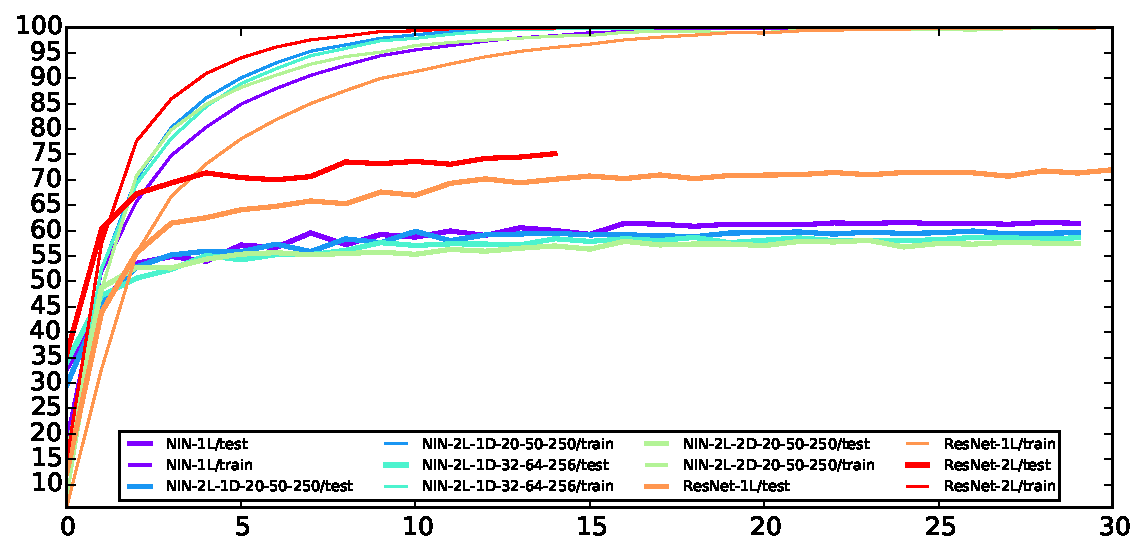
\includegraphics[width=1.0\linewidth]{figs/TCNNout}
  \caption{Temporal CNN Training and Test Error}
  \label{fig:tnntest}
\end{figure}

\begin{table}[h!]
 \caption{Best test results for a given train-test split of UCF101~\cite{ucf101}}
\centering
 \begin{tabular}{||l l||}
 \hline
 \textit{Our Results} & \\ \hline
 CNN (ResNet) & 74.97\% \\
 CNN-LSTM (ResNet) & \textbf{79.39\%} \\
 TCNN (Res2L) & 75.1\% \\ \hline
 \textit{Published Results} & \\ \hline
 LRCN~\cite{byeon2015scene} & 71.12\% \\
 C3D~\cite{stf} & \textbf{85.2\%}\footnote{Uses a specially trained ImageNet} \\
 SlowFusion~\cite{cnnvid} & 65.4\%\\ [0.5ex]
 \hline
 \end{tabular}
\end{table}

\section{Conclusion}
Perhaps the most noticeable result is that the quality of the first convolutional layer is very important. We were able to see excellent improvements in quality just by using ResNet in place of earlier ImageNet models. While we used a standard pretrained ImageNet model for this layer, we might expect improvements of 5-10\% by further training this first layer on relevant video classes. 

Data volume is very important. We had 10000 videos in our data set, but C3D was able to train on one million videos, as well as a proprietary Facebook data set.

The temporal CNN was not as effective as the LSTM model, and in fact only performed incrementally better than the raw CNN model. Performing convolutions across feature vectors is tricky. 
